\documentclass[UTF8,a4paper,12pt]{ctexart}
\usepackage{thesis-style}
\usepackage{amsmath}

\graphicspath{{../../outputs/experiment3/}}
\headermark{《金融经济数据挖掘》实验三报告}
\reporttitle{《金融经济数据挖掘》实验报告}
\reportsubtitle{实验三：基于 LGBM 的证券市场非线性预测与羊群效应因子分析}
\author{丁致宇}
\studentid{202331060205}
\major{数据科学与大数据技术}
\phone{18765788600}
\date{2026年6月}

\begin{document}

\maketitle

\begin{ustcabstract}
本报告围绕实验三“基于机器学习的非线性预测与因子解释”展开，在实验二生成的周度羊群效应指数基础上，将 $H3_t$ 与沪深300自然周收益率对齐，构造无未来信息泄露的滞后特征、滚动统计特征和时间虚拟变量，并使用 LightGBM 完成严格时序划分下的样本外预测。实验同时输出 Gain 特征重要性、SHAP 解释、残差诊断和双向传导模型，用于检验羊群效应因子是否具有非线性预测贡献，并分析市场收益与舆情羊群效应之间的反馈关系。

实验共得到 50 行自然周对齐样本，日期范围为 2014-10-20 至 2015-10-25；特征工程后可建模样本为 45 行，其中训练集 36 行、测试集 9 行。正向模型使用 $H3_t$ 与 $P_t$ 的历史滞后和滚动统计特征预测当周沪深300收益率，测试集 MSE 为 0.003503，MAE 为 0.036376，$R^2=-0.5398$，IC 为 0.1526，方向准确率为 55.56\%。反向模型使用历史收益率预测后续 $H3_t$，测试集 $R^2=0.0850$，IC 为 0.7333，方向准确率为 77.78\%。结果表明，在当前样本规模下，羊群效应对收益率的样本外预测能力需要谨慎解释，但收益变化对后续舆情羊群强度的反馈更明显，体现出一定金融反身性。
\end{ustcabstract}
\keywords{羊群效应；沪深300；LightGBM；SHAP；非线性预测；金融反身性}

\clearpage
\tableofcontents
\clearpage

\section{实验要求理解与总体设计}

实验三承接实验二输出的羊群效应指数，核心任务不是检验同期相关性，而是判断历史舆情羊群效应能否为未来市场收益提供样本外预测信息。为避免未来函数，本实验将所有用于正向预测的情绪变量都处理为滞后项或历史滚动统计量，不使用同期 $H3_t$ 直接预测同期收益。

本实验包含三条主线。第一，完成实验二羊群效应指数与沪深300日度价格数据的自然周对齐，并计算周收益率；第二，构造符合时序预测要求的机器学习特征，使用 LightGBM 完成样本外预测；第三，利用 Gain、SHAP、残差诊断和反向建模解释因子贡献，判断“舆情影响收益”和“收益反馈舆情”两条链路的相对强弱。

整体运行入口为：
\begin{CodeBlock}
python -m experiment3.main
\end{CodeBlock}

实验三代码位于 \path{experiment3/} 目录，输入数据来自 \path{outputs/experiment2/weekly_herd_index.csv} 与 \path{data/experiment2/raw/} 目录下的沪深300日价格指数文件，运行结果统一保存到 \path{outputs/experiment3/}。

\section{数据来源与样本构造}

\subsection{输入数据}

羊群效应输入文件为实验二生成的 \path{weekly_herd_index.csv}，其中核心字段包括周度交易日期、乐观情绪比例 $P_t$、情绪偏离度 $H1_t$、分歧度 $H2_t$ 和综合羊群效应指数 $H3_t$。市场数据使用沪深300日度价格指数，先按自然周聚合为周收盘价，再计算自然周收益率。

周收益率定义为：
\begin{equation}
Ret_t=\frac{Close_t-Close_{t-1}}{Close_{t-1}}.
\end{equation}

由于实验二的羊群效应指数按交易周生成，而沪深300收益率在本实验中按自然周生成，程序先将二者转换到自然周结束日口径，再做内连接，保证同一行样本中 $H3_t$、$P_t$ 与 $Ret_t$ 的时间标签一致。

\subsection{样本审计}

\begin{table}[H]
    \centering
    \caption{实验三数据处理摘要}
    \label{tab:data-summary}
    \begin{tabular}{lr}
        \toprule
        项目 & 数值 \\
        \midrule
        羊群效应自然周样本行数 & 50 \\
        沪深300自然周收益率样本行数 & 621 \\
        内连接后对齐样本行数 & 50 \\
        对齐日期范围 & 2014-10-20 至 2015-10-25 \\
        对齐后关键字段缺失单元格数 & 0 \\
        特征工程后可建模样本行数 & 45 \\
        训练集样本行数 & 36 \\
        测试集样本行数 & 9 \\
        \bottomrule
    \end{tabular}
\end{table}

表 \ref{tab:data-summary} 显示，本实验最终进入机器学习建模的样本较少，因此报告不仅给出传统误差指标，也同时观察 IC、方向准确率、特征贡献和残差分布，避免只依赖单一指标得出过强结论。

\section{特征工程与质量控制}

\subsection{特征设计}

正向预测任务的标签为当周沪深300收益率 $Ret_t$。特征集合包括 $H3$ 的 1 至 5 期滞后、$H3$ 的 3 周与 5 周滚动均值和标准差、$P_t$ 的 1 至 3 期滞后、$P_t$ 的 3 周滚动均值，以及月份和季度虚拟变量。可形式化表示为：
\begin{equation}
X_t=\{H3_{t-1},\ldots,H3_{t-5},Roll(H3)_{t-1},P_{t-1},P_{t-2},P_{t-3},TimeDummy_t\}.
\end{equation}

这里的滚动统计量均只使用历史窗口计算，不包含被预测周的同期信息。反向预测任务用于检验金融反身性，使用历史沪深300收益率预测后续 $H3_t$，从而比较“舆情到收益”和“收益到舆情”的样本外表现。

\subsection{质量检查}

\begin{table}[H]
    \centering
    \scriptsize
    \caption{实验三质量检查结果}
    \label{tab:quality-checks}
    \begin{tabular}{L{0.28\textwidth}cL{0.50\textwidth}}
        \toprule
        检查项 & 结果 & 说明 \\
        \midrule
        自然周对齐后无关键缺失 & True & $H3_t$、$P_t$、$Ret_t$ 均完整。 \\
        自然周日期单调递增 & True & 所有样本按自然周结束日升序排列。 \\
        特征工程后无缺失 & True & 滞后与滚动特征首部缺失已剔除。 \\
        未使用同期 $H3_t$ 作为正向特征 & True & 正向预测只使用 $H3_t$ 的历史滞后和历史滚动统计。 \\
        样本外测试集存在 & True & 可建模样本 45 行，按时间顺序切分训练和测试。 \\
        \bottomrule
    \end{tabular}
\end{table}

\begin{figure}[H]
    \centering
    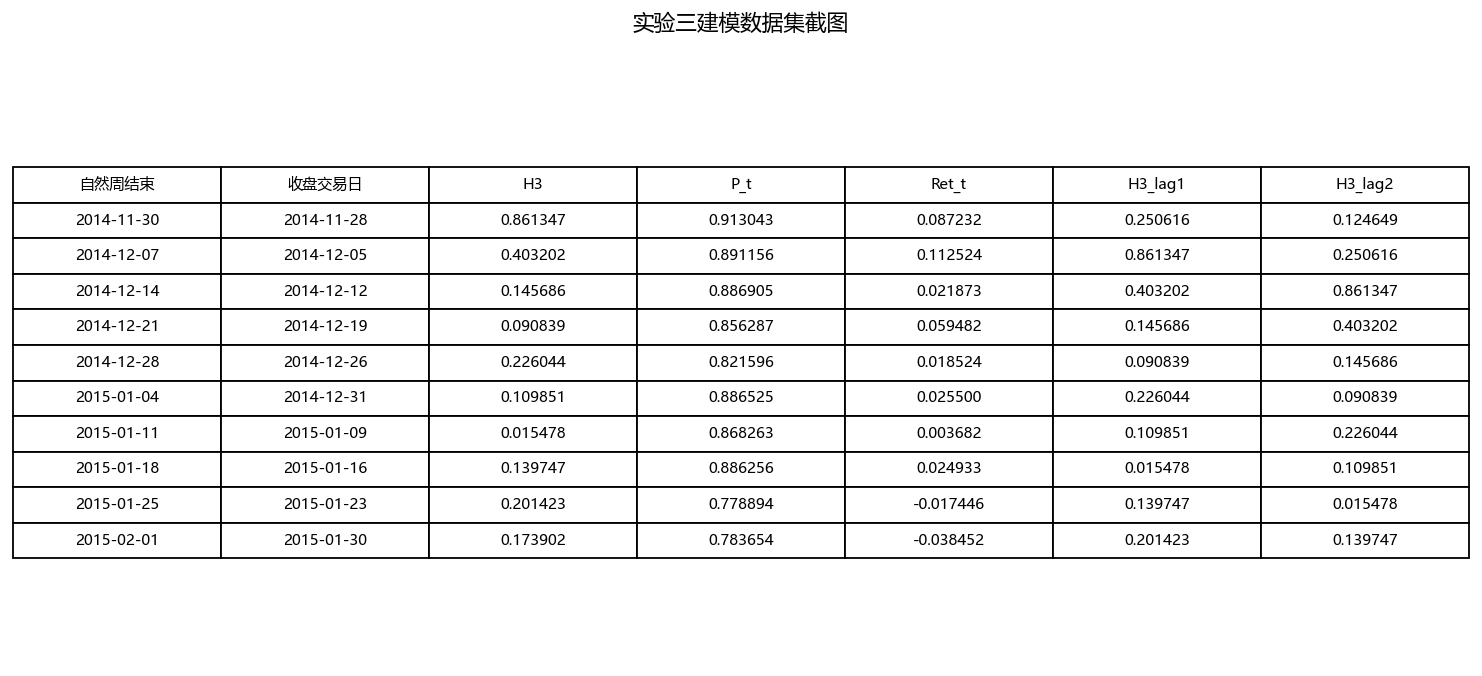
\includegraphics[width=0.96\textwidth]{modeling_dataset_table.png}
    \caption{实验三建模数据集截图}
    \label{fig:modeling-dataset}
\end{figure}

图 \ref{fig:modeling-dataset} 展示了建模数据集中 $H3_t$、$P_t$、$Ret_t$ 及滞后特征的组织方式。首部缺失来自滞后和滚动窗口构造，程序在建模前统一剔除这些行。

\section{LightGBM 建模方法}

\subsection{时序切分}

实验采用时间顺序切分训练集和测试集，而不是随机切分。原因在于金融预测任务必须模拟真实样本外环境：模型只能利用历史样本训练，然后预测未来样本。若随机切分，未来阶段的数据会进入训练集，从而高估模型表现。

在 45 行可建模样本中，前 36 行作为训练集，后 9 行作为测试集。超参数选择只在训练窗口内部完成，测试集仅用于最终评价。

\subsection{评价指标}

回归误差使用 MSE、MAE、RMSE 和 $R^2$ 衡量；排序关系使用 IC 衡量；方向信号使用方向准确率衡量。$R^2$ 的定义为：
\begin{equation}
R^2=1-\frac{\sum_{i=1}^{n}(y_i-\hat{y}_i)^2}{\sum_{i=1}^{n}(y_i-\bar{y})^2}.
\end{equation}

当 $R^2$ 为负时，说明模型样本外误差大于直接使用测试集均值作为预测基准的误差。金融收益率噪声较强，因此本实验同时报告 IC 和方向准确率，补充观察模型是否存在排序或涨跌方向上的弱信号。

\section{样本外预测结果}

\begin{table}[H]
    \centering
    \scriptsize
    \caption{正向与反向 LightGBM 测试集指标}
    \label{tab:model-metrics}
    \resizebox{\textwidth}{!}{%
    \begin{tabular}{L{0.27\textwidth}rrrrrrrr}
        \toprule
        方向 & MSE & MAE & RMSE & $R^2$ & IC & 方向准确率 & 训练 & 测试 \\
        \midrule
        $H3$ 滞后特征 $\rightarrow$ 沪深300周收益率 & 0.003503 & 0.036376 & 0.059187 & -0.539814 & 0.152564 & 0.555556 & 36 & 9 \\
        沪深300滞后收益率 $\rightarrow$ $H3$ & 0.059075 & 0.139555 & 0.243054 & 0.085004 & 0.733333 & 0.777778 & 36 & 9 \\
        \bottomrule
    \end{tabular}}
\end{table}

表 \ref{tab:model-metrics} 显示，正向模型测试集 $R^2=-0.5398$，说明在严格样本外条件下，羊群效应因子预测周收益率的误差仍大于均值基准。不过，IC 为 0.1526，方向准确率为 55.56\%，说明模型在排序和方向上仍存在一定弱信号。反向模型 $R^2=0.0850$，IC 为 0.7333，方向准确率为 77.78\%，明显强于正向模型，表明市场收益变化对后续舆情羊群强度的反馈更稳定。

\begin{figure}[H]
    \centering
    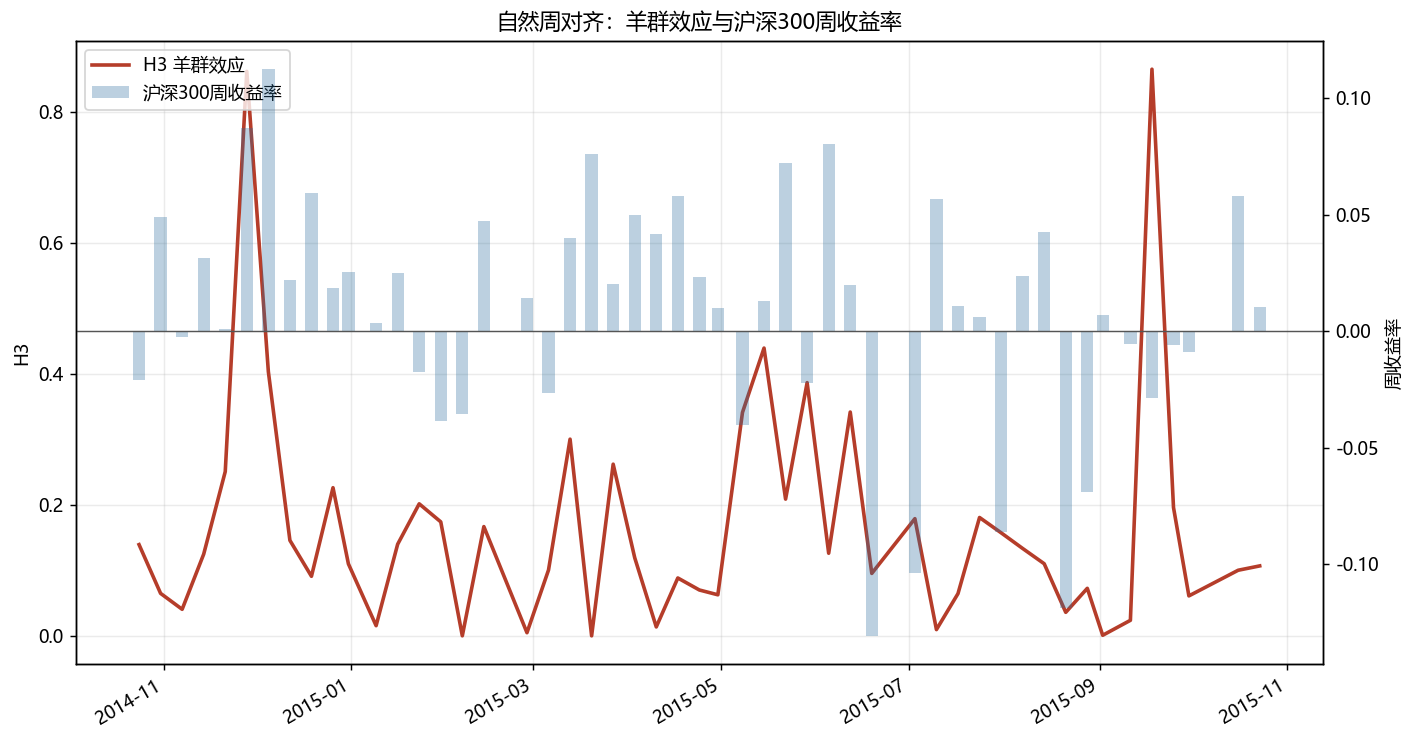
\includegraphics[width=0.96\textwidth]{market_herd_timeseries.png}
    \caption{自然周对齐后的羊群效应指数与沪深300周收益率}
    \label{fig:market-herd}
\end{figure}

\begin{figure}[H]
    \centering
    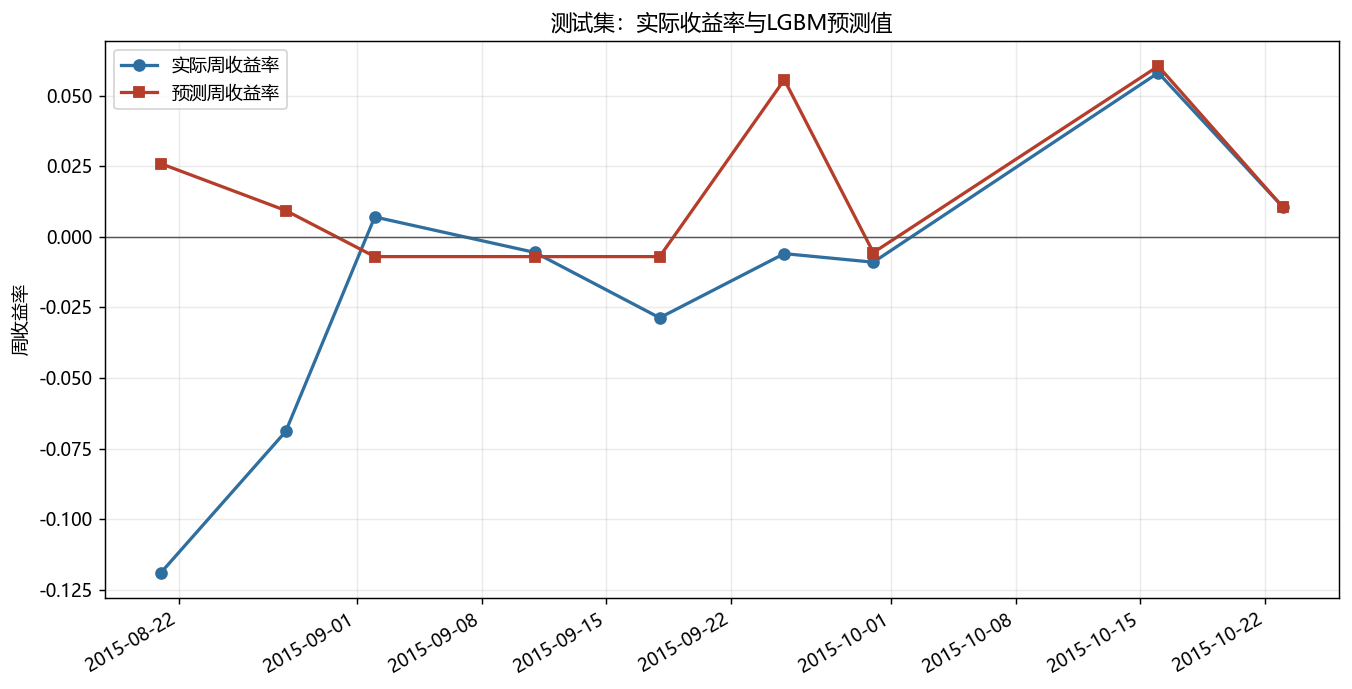
\includegraphics[width=0.92\textwidth]{prediction_vs_actual.png}
    \caption{测试集实际收益率与 LightGBM 预测值}
    \label{fig:pred-vs-actual}
\end{figure}

图 \ref{fig:market-herd} 展示了对齐后 $H3_t$ 与沪深300周收益率的时间变化。图 \ref{fig:pred-vs-actual} 进一步说明，正向模型在部分测试周可以捕捉方向变化，但对极端波动的幅度刻画不足，这也是 $R^2$ 为负的重要原因。

\section{因子贡献与 SHAP 解释}

\subsection{Gain 特征重要性}

LightGBM 的 Gain 重要性衡量特征在树分裂中带来的损失下降贡献。实验结果显示，$H3$ 类特征 Gain 总贡献占比为 40.84\%，$P_t$ 辅助情绪特征贡献占比为 57.71\%，时间虚拟变量贡献占比为 1.45\%。这说明模型主要依赖情绪相关变量，而不是月份或季度虚拟变量。

\begin{table}[H]
    \centering
    \scriptsize
    \caption{LightGBM Gain 特征重要性前 8}
    \label{tab:gain-importance}
    \begin{tabular}{lrrr}
        \toprule
        特征 & Gain & Split & Gain 占比 \\
        \midrule
        \texttt{P\_t\_roll\_mean\_3} & 0.183076 & 15 & 0.281610 \\
        \texttt{H3\_roll\_std\_3} & 0.126210 & 14 & 0.194138 \\
        \texttt{P\_t\_lag2} & 0.080444 & 27 & 0.123740 \\
        \texttt{P\_t\_lag3} & 0.072030 & 25 & 0.110798 \\
        \texttt{H3\_lag1} & 0.062926 & 25 & 0.096793 \\
        \texttt{P\_t\_lag1} & 0.039636 & 21 & 0.060969 \\
        \texttt{H3\_roll\_std\_5} & 0.034726 & 21 & 0.053416 \\
        \texttt{H3\_lag2} & 0.014847 & 18 & 0.022837 \\
        \bottomrule
    \end{tabular}
\end{table}

\begin{figure}[H]
    \centering
    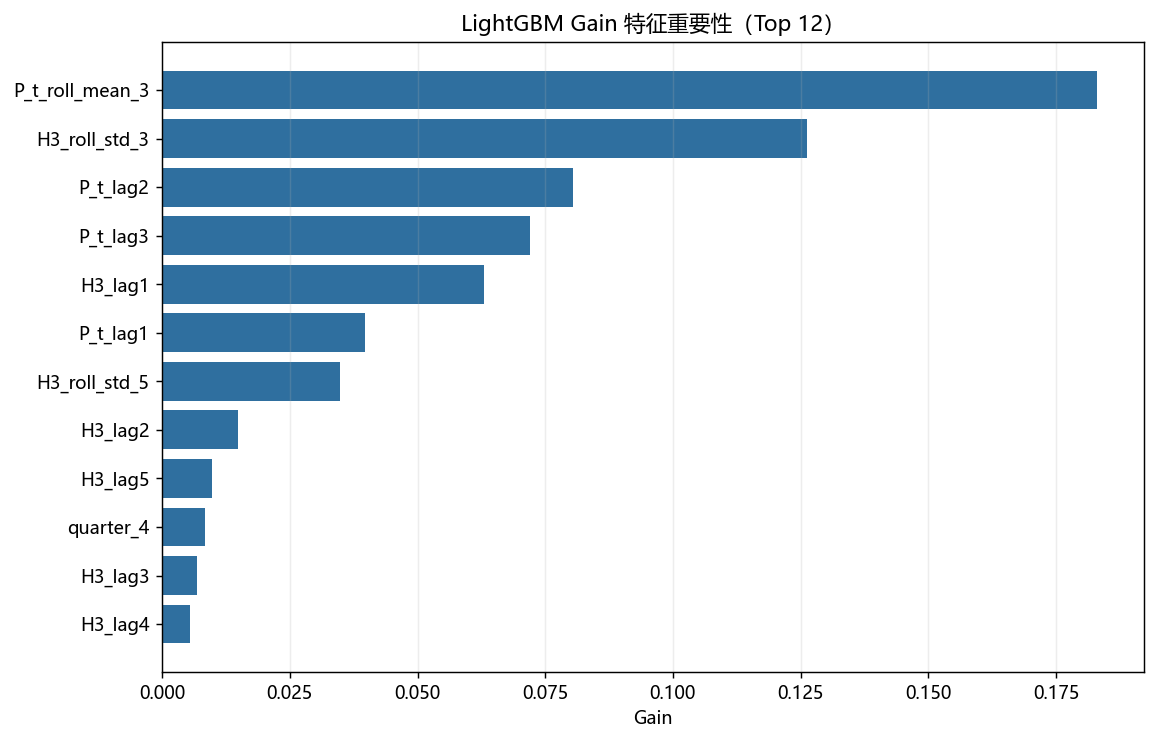
\includegraphics[width=0.88\textwidth]{feature_importance_gain.png}
    \caption{LightGBM Gain 特征重要性}
    \label{fig:gain}
\end{figure}

按 Gain 排序，最优 $H3$ 滞后特征为 \texttt{H3\_lag1}，说明最近一期羊群效应变化对模型分裂贡献最大。与此同时，\texttt{H3\_roll\_std\_3} 排在全部特征第二位，说明羊群效应本身的短期波动强度也是重要信号。

\subsection{SHAP 非线性解释}

SHAP 重要性从局部解释角度度量特征对预测值的平均绝对影响。与 Gain 不同，SHAP 更关注特征在实际预测样本中的边际贡献。

\begin{table}[H]
    \centering
    \scriptsize
    \caption{SHAP 特征重要性前 8}
    \label{tab:shap-importance}
    \begin{tabular}{lrr}
        \toprule
        特征 & 平均绝对 SHAP & SHAP 占比 \\
        \midrule
        \texttt{H3\_roll\_std\_3} & 0.010503 & 0.212484 \\
        \texttt{P\_t\_lag2} & 0.008234 & 0.166585 \\
        \texttt{H3\_roll\_std\_5} & 0.006994 & 0.141497 \\
        \texttt{P\_t\_lag1} & 0.005554 & 0.112360 \\
        \texttt{P\_t\_lag3} & 0.003417 & 0.069139 \\
        \texttt{P\_t\_roll\_mean\_3} & 0.003105 & 0.062809 \\
        \texttt{H3\_lag5} & 0.002752 & 0.055686 \\
        \texttt{quarter\_4} & 0.002497 & 0.050511 \\
        \bottomrule
    \end{tabular}
\end{table}

\begin{figure}[H]
    \centering
    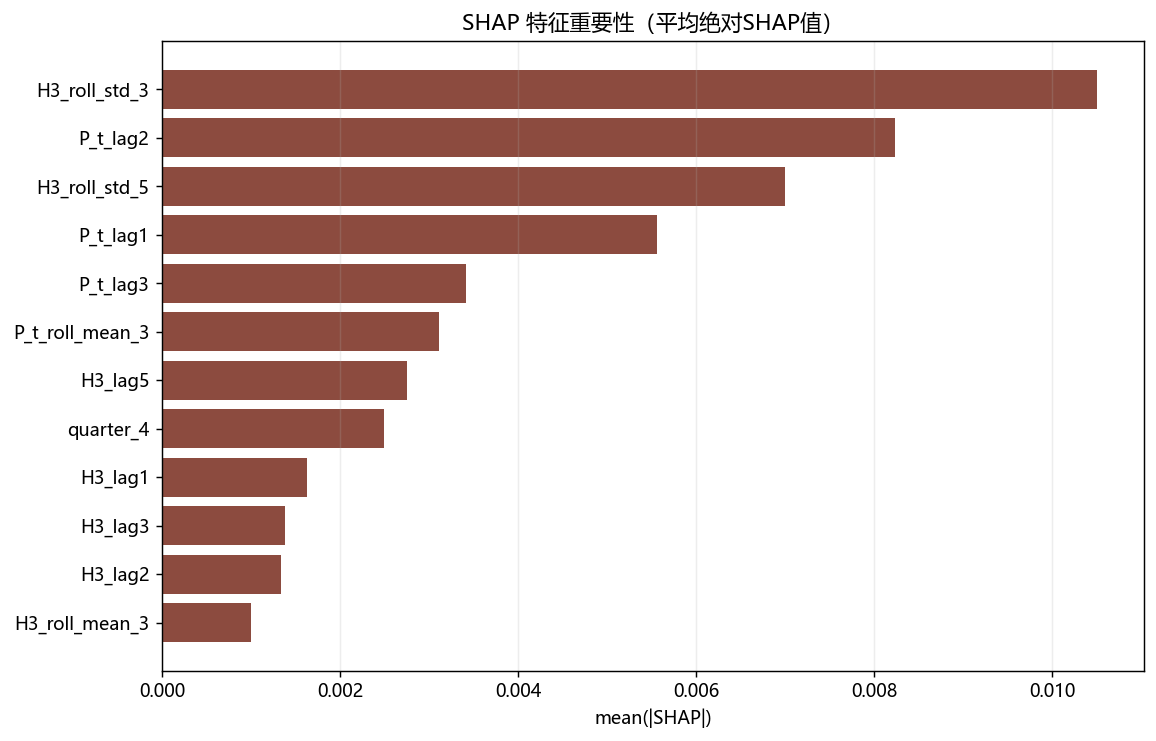
\includegraphics[width=0.88\textwidth]{shap_feature_importance.png}
    \caption{SHAP 特征重要性}
    \label{fig:shap-importance}
\end{figure}

\begin{figure}[H]
    \centering
    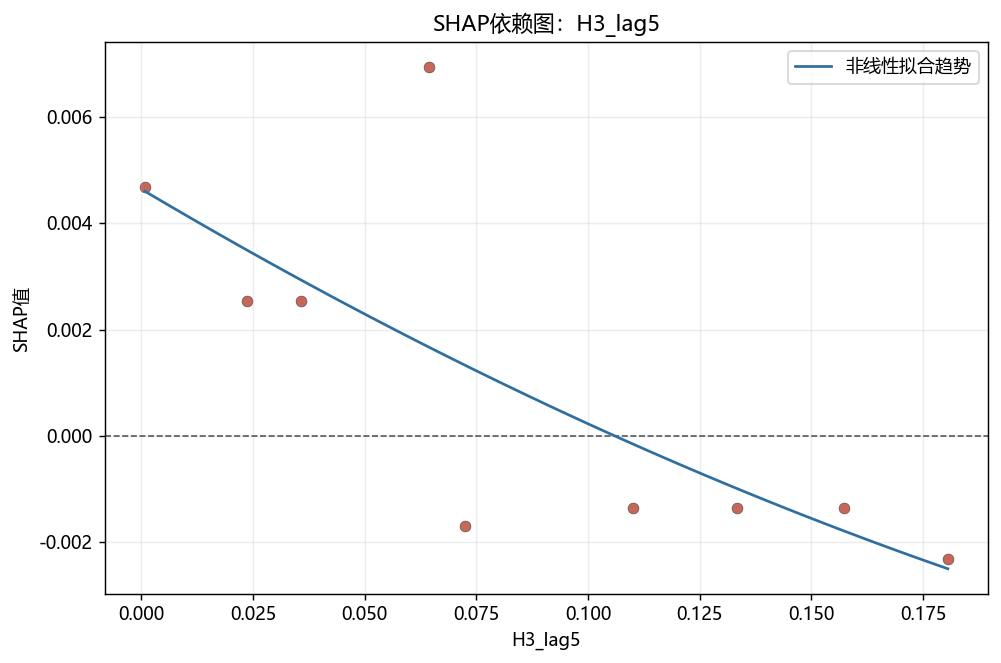
\includegraphics[width=0.78\textwidth]{shap_dependence_best_lag.png}
    \caption{最优 H3 滞后因子的 SHAP 依赖图}
    \label{fig:shap-dependence}
\end{figure}

按 SHAP 排序，贡献最高的 $H3$ 相关特征为 \texttt{H3\_roll\_std\_3}，最优单一滞后项为 \texttt{H3\_lag5}。这与 Gain 中 \texttt{H3\_lag1} 最优并不矛盾：Gain 更关注树分裂过程，SHAP 更关注预测样本中的边际影响。图 \ref{fig:shap-dependence} 如果呈现弯曲或分段形态，则说明羊群效应对收益率的影响并非固定线性斜率，而可能存在阈值效应。

\section{残差诊断}

\begin{table}[H]
    \centering
    \caption{测试集残差描述统计}
    \label{tab:residual}
    \begin{tabular}{lr}
        \toprule
        指标 & 数值 \\
        \midrule
        残差均值 & -0.032930 \\
        残差标准差 & 0.049180 \\
        残差最小值 & -0.144697 \\
        残差最大值 & 0.014041 \\
        残差绝对值均值 & 0.036376 \\
        \bottomrule
    \end{tabular}
\end{table}

\begin{figure}[H]
    \centering
    
\includegraphics[width=0.92\textwidth]{residual_timeseries.png}
    \caption{测试集残差时序图}
    \label{fig:residual-timeseries}
\end{figure}

\begin{figure}[H]
    \centering
    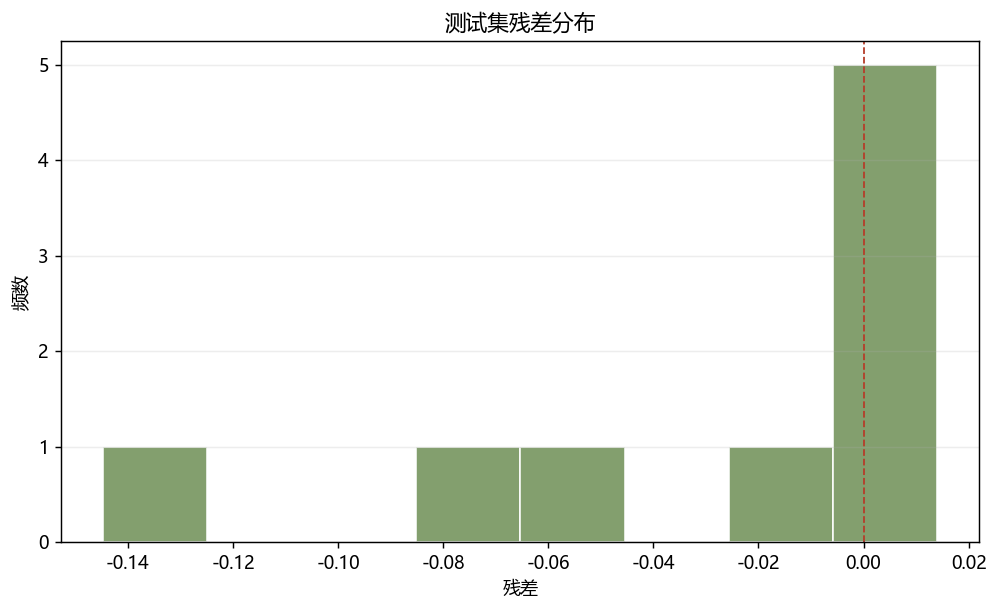
\includegraphics[width=0.70\textwidth]{residual_distribution.png}
    \caption{测试集残差分布}
    \label{fig:residual-distribution}
\end{figure}

测试集残差均值为 -0.032930，说明模型整体存在一定高估收益的倾向。残差最小值为 -0.144697，表明个别测试周出现了较明显的负向误差。金融市场收益容易受到政策、流动性和突发事件影响，仅依赖舆情羊群效应难以完全解释这些极端波动。

\section{双向传导与金融反身性}

金融反身性强调市场价格与投资者认知之间存在相互影响。为了检验这一点，本实验在正向预测之外构造反向模型：使用沪深300历史收益率预测后续羊群效应指数 $H3_t$。

\begin{table}[H]
    \centering
    \scriptsize
    \caption{双向建模结果对比}
    \label{tab:bidirectional}
    \resizebox{\textwidth}{!}{%
    \begin{tabular}{L{0.32\textwidth}rrrrrrl}
        \toprule
        方向 & MSE & MAE & RMSE & $R^2$ & IC & 方向准确率 & 最优滞后 \\
        \midrule
        $H3$ 滞后特征 $\rightarrow$ 沪深300周收益率 & 0.003503 & 0.036376 & 0.059187 & -0.539814 & 0.152564 & 0.555556 & \texttt{H3\_lag1} \\
        沪深300滞后收益率 $\rightarrow$ $H3$ & 0.059075 & 0.139555 & 0.243054 & 0.085004 & 0.733333 & 0.777778 & \texttt{Ret\_lag1} \\
        \bottomrule
    \end{tabular}}
\end{table}

\begin{figure}[H]
    \centering
    
\includegraphics[width=0.92\textwidth]{bidirectional_comparison.png}
    \caption{双向建模样本外效果对比}
    \label{fig:bidirectional}
\end{figure}

表 \ref{tab:bidirectional} 和图 \ref{fig:bidirectional} 表明，反向模型在 $R^2$、IC 和方向准确率上均优于正向模型。这说明在当前样本中，“收益驱动舆情”的反馈链条更明显：市场涨跌会改变新闻叙事和投资者情绪，而这些情绪再进一步影响后续市场行为。该结果并不否定羊群效应因子的研究价值，而是提示在短样本、强噪声的金融数据中，应同时关注预测链路和反馈链路。

\section{输出文件与复现说明}

实验三主要输出文件包括：
\begin{itemize}
    \item \path{aligned_weekly_dataset.csv}：自然周对齐后的 $H3_t$、$P_t$ 与沪深300收益率。
    \item \path{feature_engineering.csv}：包含滞后项、滚动统计和时间虚拟变量的特征工程表。
    \item \path{lgbm_forward_results.csv}：正向模型测试集预测结果。
    \item \path{model_metrics.csv}：正向和反向模型测试集评价指标。
    \item \path{feature_importance_gain.csv} 与 \path{shap_importance.csv}：特征贡献表。
    \item \path{experiment3.db}：SQLite 结果库。
    \item AI 代码审查与修复表、AI 交互记录和实验三代码附录：AI 辅助与代码附录材料。
\end{itemize}

报告中的图表均由程序自动生成，图片文件保存在 \path{outputs/experiment3/}。本 LaTeX 报告源文件位于 \path{Code/report/experiment3_latex/main.tex}，使用 XeLaTeX 编译。

\section{实验结论}

本实验完成了从实验二羊群效应指数到 LightGBM 非线性预测、SHAP 因子解释、残差诊断和双向传导验证的完整链路。实验结果说明，羊群效应因子在严格样本外条件下预测沪深300周收益率的能力较弱，正向模型 $R^2$ 为负，但情绪变量仍在 Gain 和 SHAP 中表现出可量化贡献，尤其是短期波动特征和滞后特征。

从双向建模看，收益率对后续羊群效应的解释力更强，说明市场价格变化会反过来塑造新闻叙事和投资者情绪。相比线性回归，LightGBM 更适合处理金融情绪变量可能存在的阈值效应、分段非线性和反馈关系；但由于样本规模较小，后续若要形成更稳健的投资结论，还需要扩展更长时间窗口并进行滚动样本外检验。

\end{document}
